\documentclass[a4paper]{article}
\usepackage{fancyhdr}
\usepackage[usenames, dvipsnames]{xcolor}
\usepackage{graphicx,hyperref,amsmath,float,subfigure,soul,caption}
\usepackage[top=3cm,bottom=3cm,left=3cm,right=3cm]{geometry}
\hypersetup{
	colorlinks,
	citecolor=black,
	filecolor=black,
	linkcolor=black,
	urlcolor=black
}
\newcommand{\HRule}{\rule{\linewidth}{0.5mm}}
\pagestyle{fancy}
\lfoot{\small \color{gray}Tom Peerdeman - 10266186}
\cfoot{\thepage}
\rfoot{\small \color{gray}Ren\'e Aparicio Sa\'ez - 10214054}
\lhead{\small \color{gray} OMP}
\begin{document}
	\begin{titlepage}
	\begin{center}
		\textsc{\Large Concurrency \& Parallel Programming}\\[0.5cm]
		\HRule \\[0,4cm]
		\textsc{\huge \bfseries OMP}
		\HRule \\[8cm]
		\begin{minipage}{0.4\textwidth}
			\begin{flushleft}\large
				\emph{Auteurs: Tom Peerdeman \& Ren\'e Aparicio Saez}\\
			\end{flushleft}
		\end{minipage}
		\begin{minipage}{0.4\textwidth}
			\begin{flushright}\large
			\emph{Datum: 19-11-2012\\\hspace{1cm}}\\
			\end{flushright}
		\end{minipage}
	\end{center}
	\end{titlepage}

  \section{Assignment 3.1 - Wave simulation}
  \subsection{Table with results}
    Tests on DAS4 are run for i\_max = 1.000.000 and t\_max = 1.000.
    The amount of omp threads used to generate the waves is increased
    to measure the difference in speed for the program.
    Each amount of threads is run 12 times. 
    The highest value and the lowest value are disregarded. 
    The remaining data is used to plot a graph.
    These tests are done without specifying scheduling,
    this is done later in the report.\\\\
    \begin{tabular}{| c | c | c | c | c | c | c | c |}
      \hline
      \multicolumn{4}{|c}{i = 1,000,000} & \multicolumn{4}{c|}{t = 1,000}\\
      \hline
\st{3.1211} & 1.43211 & 1.26944 & 0.939188 & 0.851557 & 0.623673 & 0.718125 & 0.677228\\
      \hline
3.04543 & 1.42686 & 1.29452 & 0.813184 & 0.873015 & 0.654943 & 0.756256 & \st{0.587986}\\
      \hline
\st{3.02998} & \st{1.40477} & 1.33823 & 0.813059 & 0.848276 & \st{0.593785} & 0.740096 & \st{0.694887}\\
      \hline
3.0661 & 1.4104 & 1.45341 & 0.772554 & 0.878858 & 0.670092 & 0.720322 & 0.631909\\
      \hline
3.06365 & 1.41057 & \st{1.68411} & 0.814582 & \st{0.988416} & 0.630324 & 0.736533 & 0.664366\\
      \hline
3.08719 & 1.42461 & 1.30602 & \st{0.939831} & \st{0.828244} & 0.621332 & \st{0.716592} & 0.663344\\
      \hline
3.08742 & \st{2.20822} & 1.27907 & 0.802773 & 0.91554 & 0.628798 & 0.816578 & 0.622237\\
      \hline
3.04847 & 1.41933 & 1.30155 & 0.837648 & 0.854704 & 0.617878 & 0.833466 & 0.601991\\
      \hline
3.06515 & 1.44256 & 1.45228 & 0.913682 & 0.839151 & \st{0.708951} & \st{0.845428} & 0.677083\\
      \hline
3.04467 & 1.42778 & 1.29303 & \st{0.771725} & 0.845102 & 0.66214 & 0.731911 & 0.615128\\
      \hline
3.03383 & 1.44278 & 1.32129 & 0.825917 & 0.868847 & 0.666777 & 0.736191 & 0.592873\\
      \hline
3.07641 & 1.43763 & \st{1.26484} & 0.778603 & 0.89026 & 0.571218 & 0.73283 & 0.659633\\
      \hline
      \multicolumn{8}{|l|}{Average of the remaining 10:}\\
      \hline
      3.061832 & 1.424268 & 1.330884 & 0.8311174 & 0.8664933 & 0.6306423 & 0.7523437 & 0.6399728\\
      \hline
    \end{tabular}
    \begin{center}
      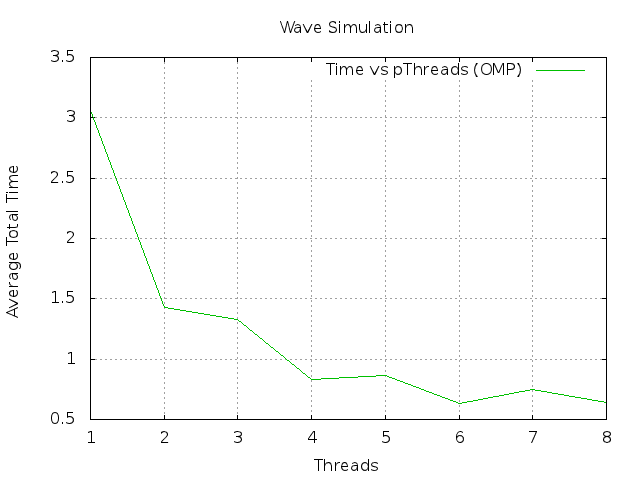
\includegraphics[width=0.9\textwidth]{speedplotsolo.png}
    \end{center}
    Apparantly the performance is better if an even number of threads is used.
  \newpage
  \subsection{Comparison between schedulers}
    OpenMP has three different types of schedulers.
    Below are the results of the different
    schedulers to calculate the wave equations. 
    If no scheduler is specified, 'static' is the standard scheduler.
    Just in case, new tests are run specifying 'static' as scheduler.
    The tests where run using i\_max = 1,000,000 and t\_max = 1,000.
    \begin{center}
      \begin{tabular}{| c | c | c |}
      \hline
      guided, 1 & dynamic, $\frac{i\_max}{num\_threads}$ & static, $\frac{i\_max}{num\_threads}$\\
      \hline
      1.34428 & 1.29205 & 0.639236\\
      \hline
      1.33937 & 1.34629 & 0.652469\\
      \hline
      1.35234 & 1.32758 & 0.646157\\
      \hline
      1.33636 & 1.2953 & 0.638384\\
      \hline
      1.30415 & 1.33798 & 0.681617\\
      \hline
      1.3897 & 1.34237 & 0.69578\\
      \hline
      1.37503 & 1.20245 & 0.650952\\
      \hline
      1.33084 & 1.24136 & 0.685962\\
      \hline
      \multicolumn{3}{|l|}{Average of the runs:}\\
      \hline
      1.35120375 & 1.31465 & 0.661319625\\
      \hline
      \end{tabular}
    \end{center}
    Tests using the 'guided' scheduler, but with a bigger smallest chunk resulted
    in slower preformance or equal preformance. The best scheduler for this equation
    is the 'static' scheduler.
    
    
  \subsection{Comparison to normal pThreads}
    When comparing the results, it becomes clear that OMP (without any specified scheduler) is faster then the usual pThread parallelisation method.\\\\
    \begin{tabular}{| l | c | c | c | c | c | c | c | c |}
      \hline
      \multicolumn{9}{|c|}{Average of 10 runs:}\\
      \hline
      & 1 thread & 2 threads & 3 threads & 4 threads & 5 threads & 6 threads & 7 threads & 8 threads\\
      \hline
      pThreads & 3.788914 & 1.701978 & 1.713576 & 0.9564147 & 1.173655 & 0.7479494 & 0.89525656 & 0.6777506\\
      \hline
      OMP & 3.061832 & 1.424268 & 1.330884 & 0.8311174 & 0.8664933 & 0.6306423 & 0.7523437 & 0.6399728\\
      \hline
    \end{tabular}
    \begin{center}
      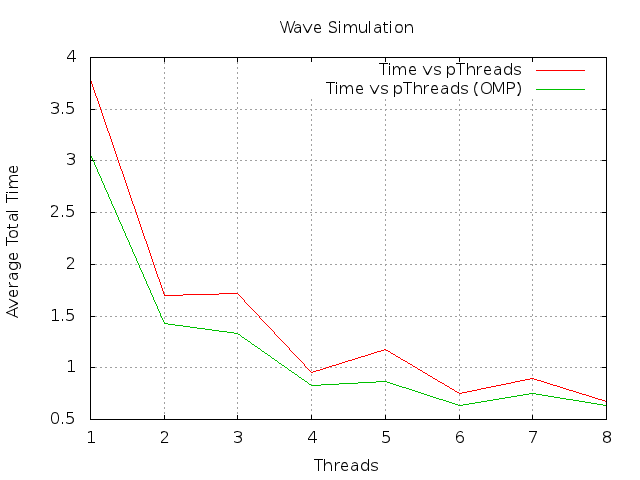
\includegraphics[width=0.9\textwidth]{speedplot.png}
    \end{center}
\newpage
\section{Assignment 3.2 - Mandelbrot set}
\subsection{Finding a suitable resolution}
	For comparing different code approaches a good resolution is needed.
	If a low resolution is chosen, so that dyx is low, the program will finish very quick.
	If we want to make a comparison this wont work very well.
	The difference in results based on the change of code will be overwhelmed by the difference in results due to changes in cpu-load.
	A too high resolution is also unwanted, for a good comparison multiple runs are required.
	If the program takes too long too finish less runs can be done.
	The resolution is experimentally found.
	Starting at 0.005 we found that the program run times were just too low.
	Eventually we settled at a value of 0.002, with this resolution running on normal computers a good difference could be seen.
	However when we ran the program at das4 the multiple cores kicked in, so we had to lower the resolution to 0.001 to be in the clear.
	

\subsection{Work schedulers}
	The mandelbrot application isn't an application with a fixed amount of instructions in each loop.
	In the loop a while statement sits, which runs a couple of times depending on the data.
	So if each thread get a fixed amount of points to process some threads will get points that exit the while loop quickly, while a other thread can get points that take a long time to exit the while loop.
	It will be clear that these threads wont finish their portion of points a the same time, on thread will be finished before the other one.
	In the static scheduling all the work is divided before starting the threads.
	The thread that is finished before the other threads will just sit there and do nothing because it cannot steal points from other threads.
	The dynamic scheduler doesn't divide all the point in the begin. Each thread gets a couple of points assigned.
	if a thread finishes it can request more points to process. The dynamic scheduler will therefore be perfect for our goal.
	We can see from table \ref{table:mandel_schedulers} that this works in practice as well.
	The dynamic scheduler is much faster than the static scheduler.
	The guided scheduler also works quite good, but not as good as the dynamic one.
	
\begin{table}[h]
	\caption{Running mandel with output using different schedulers.\\The resolution is 0.001.}
	\label{table:mandel_schedulers}
	\begin{center}
		\begin{tabular}{| c | c | c |}
			\hline
			Dynamic & Static & Guided\\ 
			\hline
			0,470178 & 0,757189 & 0,501167\\ 
			0,476920 & 0,768196 & 0,503846\\ 
			0,481399 & 0,784334 & 0,501800\\ 
			0,482518 & 0,806455 & 0,502887\\ 
			0,490624 & 0,797248 & 0,523842\\ 
			0,508222 & 0,782431 & 0,539778\\ 
			0,504364 & \st{0,821781} & 0,539267\\ 
			0,533801 & 0,805446 & 0,552913\\ 
			0,528836 & 0,816622 & \st{0,577115}\\ 
			0,481194 & 0,818687 & 0,554339\\ 
			0,479515 & 0,765153 & 0,501227\\ 
			0,479229 & 0,771336 & 0,500563\\ 
			0,482719 & 0,765416 & \st{0,487623}\\ 
			\st{0,464592} & 0,786886 & 0,490257\\ 
			0,500019 & \st{0,749763} & 0,540523\\ 
			0,482475 & 0,764995 & 0,530378\\ 
			0,521944 & 0,769605 & 0,552142\\ 
			0,523241 & 0,818235 & 0,554799\\ 
			\st{0,533844} & 0,814846 & 0,503505\\ 
			0,483639 & 0,769063 & 0,503250\\ 
			\hline
			0,495047 & 0,786786 & 0,522027\\ 
			\hline
		\end{tabular}
	\end{center}
\end{table}

\subsection{Best run times}
	In table \ref{table:mandel_nout_o3} we can see the runtimes of the program without any output.
	In this case the O2 compiler flag is used.
	As we can see the program finishes very quick using the parallel approach and the dynamic scheduler.
	This is not a valid result because the compiler optimizes the code by removing unused code.
	In our case of no output at all, all the parallel code can be removed.
	Most of the remaining time will be starting up the threads which terminate immediately.
	The sequential code doesn't finish instant, this could be caused by the the openmp compiler.
	The openmp compiler could be more reserved for optimizing sequential code than the normal compiler.\\
	To get some real results we disabled the compiler optimalisations by removing the O2 flag.
	The results are shown in table \ref{table:mandel_nout_schedulers}.
	We can see that the times are not as good as in table \ref{table:mandel_schedulers}, this is because the compiler optimalisations are turned off.
	If we compare the sequential code in table \ref{table:mandel_nout_schedulers} with the sequential code using the compiler optimalisations in table \ref{table:mandel_nout_o3}
	we see the difference in run time caused by the compiler optimalisations is 0.53 sec.
	This difference is almost 50\% of the runtime of the unoptimized sequential code.\\
	
	\begin{table}[h]
		\caption{Running mandel without output and with compiler optimalisations.\\The resolution is 0.001.}
		\label{table:mandel_nout_o3}
		\begin{center}
			\begin{tabular}{| c | c |}
				\hline
				Sequential & Dynamic\\ 
				\hline
				0,651594 & 0,0818824\\ 
				0,651586 & 0,0818495\\ 
				0,651614 & 0,0818448\\ 
				0,651548 & 0,0834362\\ 
				0,651608 & 0,0818953\\ 
				0,651556 & 0,0818747\\ 
				0,651563 & \st{0,0818330}\\ 
				\st{0,651443} & \st{0,0840247}\\ 
				0,651496 & 0,0818772\\ 
				\st{0,651625} & 0,0818726\\ 
				\hline
				0,651571 & 0,0820670\\ 
				\hline
			\end{tabular}
		\end{center}
	\end{table}
	
	\noindent The unoptimalised code still runs best using the dynamic scheduler. 
	The best time for the unoptimalized code is therefore a run with the dynamic scheduler wit a time of 0,7672 sec.
	This time is close followed by a time from the guided scheduler: 0,768145 sec.
	As we can see the time from the guided scheduler is not very close to the other times from the guided scheduler.
	The time with optimalisations and with output is as mentioned earlier from the dynamic scheduler: 0,464592 sec.

	\begin{table}
		\caption{Running mandel without output using different schedulers and sequential.\\The resolution is 0.001 and no compiler optimalizations are used.}
		\label{table:mandel_nout_schedulers}
		\begin{center}
			\begin{tabular}{| c | c | c | c |}
				\hline
				Sequential & Dynamic & Static & Guided\\ 
				\hline
				1,18568 & 0,768784 & 0,826720 & 0,772624\\ 
				\st{1,18586} & 0,769449 & 0,842050 & 0,776406\\ 
				1,18567 & 0,76848 & 0,842205 & 0,778630\\ 
				1,18552 & 0,77718 & 0,829137 & 0,787260\\ 
				1,18568 & 0,774852 & 0,852485 & 0,788156\\ 
				1,18566 & 0,791338 & 0,840201 & 0,782334\\ 
				1,18560 & 0,771359 & 0,83925 & 0,782231\\ 
				\st{1,18547} & 0,773696 & 0,853402 & 0,782055\\ 
				1,18560 & 0,796883 & \st{0,926374} & \st{0,814374}\\ 
				1,18549 & 0,771051 & 0,849094 & 0,776001\\ 
				1,18570 & 0,770216 & \st{0,807327} & 0,780678\\ 
				1,18569 & \st{0,7672} & 0,836319 & 0,787131\\ 
				1,18566 & 0,770971 & 0,843178 & 0,780753\\ 
				1,18570 & 0,776165 & 0,849376 & 0,784131\\ 
				1,18550 & 0,770631 & 0,851354 & 0,776077\\ 
				1,18562 & 0,775439 & 0,860626 & 0,789332\\ 
				1,18573 & 0,795864 & 0,853210 & 0,778719\\ 
				1,18562 & \st{0,797003} & 0,856143 & 0,779836\\ 
				1,18549 & 0,771624 & 0,852250 & 0,785575\\ 
				1,18554 & 0,770685 & 0,847866 & \st{0,768145}\\ 
				\hline
				1,18562 & 0,775815 & 0,845826 & 0,781552\\ 
				\hline
			\end{tabular}
		\end{center}
	\end{table}
\end{document}
